\documentclass[tikz,border=10pt]{standalone}
\usepackage{tkz-graph}
\usepackage{amsmath,amssymb}
\usepackage{xcolor}
\usetikzlibrary{calc}
\usetikzlibrary{positioning}
\usetikzlibrary{snakes}
\usetikzlibrary{arrows.meta}
\usetikzlibrary{decorations.pathreplacing}
\usepackage{pgfplots}

\definecolor{mymauve}{rgb}{0.58,0,0.82}
\definecolor{mygold}{HTML}{B8860B}
\definecolor{mynavy}{HTML}{000080}

\definecolor{olivegreen}{rgb}{0,0.6,0}

\colorlet{myred}{red!80!black}
\colorlet{myblue}{blue!80!black}
\colorlet{mygreen}{green!60!black}
\colorlet{myorange}{orange!70!red!60!black}
\colorlet{mydarkred}{red!30!black}
\colorlet{mydarkblue}{blue!40!black}
\colorlet{mydarkgreen}{green!30!black}

% COLORS
\colorlet{mylightred}{red!95!black!30}
\colorlet{mylightblue}{blue!95!black!30}
\colorlet{mylightgreen}{green!95!black!30}

\begin{document}

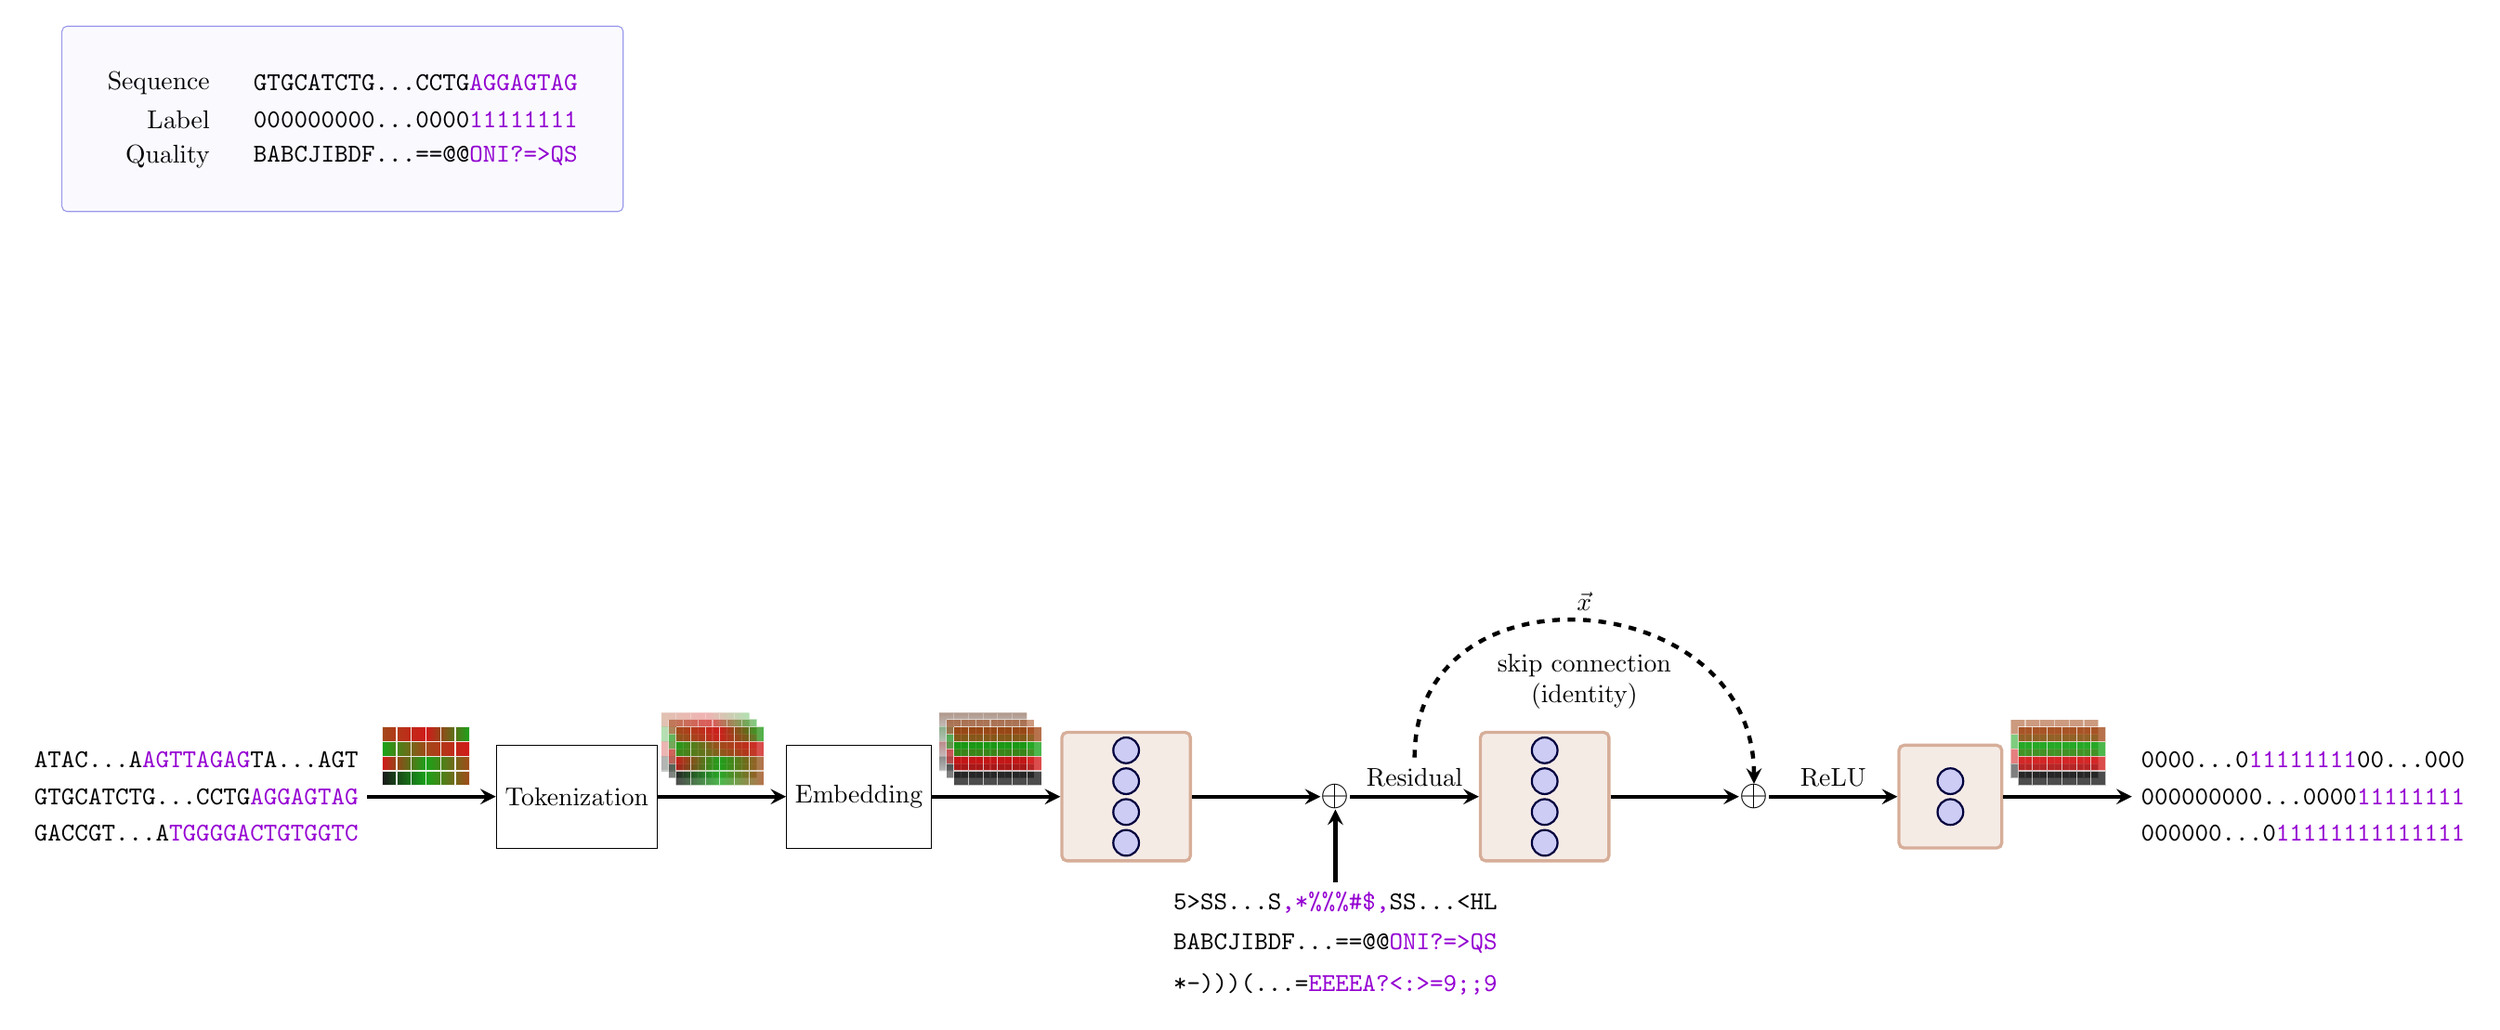
\begin{tikzpicture}[
		neuron/.style={circle, draw, fill=black!10, minimum size=1em},
		node/.style={thick,circle,draw=myblue,minimum size=1em,inner sep=0.5,outer sep=0.5},
		node hidden/.style={node,blue!20!black,draw=myblue!30!black,fill=myblue!20},
		node embed/.style={thick, circl, minimum size=0.5em, fill=mygreen!20,draw=mygreen!30!black},
	]

	\begin{scope}[scale=1, local bounding box=seqbox]
		\node (seq) at (0,0) {\tt GTGCATCTG\dots CCTG\textcolor{mymauve}{AGGAGTAG}};
		\node (label) at (0,-0.5) {\tt 000000000\dots 0000\textcolor{mymauve}{11111111}};
		\node (qual) at (0,-1) {\tt BABCJIBDF\dots ==@@\textcolor{mymauve}{ONI?=>QS}};
		% add name seq and label to the left part of the sequence
		\node[left = 1em of seq] (seq_text)  {Sequence};
		\node[left = 1em of label]  (label_text) {Label};
		\node[left = 1em of qual] (qual_text)  {Quality};
		% add a box around the sequence 
		\draw [myblue!40, fill=myblue, fill opacity=0.02,rounded corners=2]  ($(seq_text.north west) + (-0.5, 0.5)$) rectangle ($(qual.south east) + (0.5, -0.5)$);
	\end{scope}

	% add model architecture                             relu     residual ----------------
	%                                                                                     | relu
	% seq -> tokenization -> embedding ->  linear layer ------> + ------> linear layer -> + -----> output
	%                                                           |
	%                                                          qual 
	\begin{scope}[shift={($(seqbox.south)+(-2,-8)$)}, scale=1, local bounding box=modelbox1]
		% define box size 
		\def\boxsize{4em}
		\def\boxdist{5em}
		\def\boxcolor{myorange}

		% add seq -> tokenization
		\node (seq) at (0,0) { \tt GTGCATCTG\dots CCTG\textcolor{mymauve}{AGGAGTAG}};
		\node[below = 1pt of seq] (seq2)  { \tt GACCGT\dots A\textcolor{mymauve}{TGGGGACTGTGGTC}};
		\node[above = 1pt of seq] (seq3)  { \tt ATAC\dots A\textcolor{mymauve}{AGTTAGAG}TA\dots AGT};

		% add tokenization as rectangle
		\node[right = \boxdist of seq] (token) [rectangle, draw, minimum size=\boxsize] {Tokenization};
		% add embedding as rectangle
		\node[right = \boxdist of token] (embed) [rectangle, draw, minimum size=\boxsize] {Embedding};


		\node[\boxcolor!40, right = \boxdist of embed, draw, fill=\boxcolor, fill opacity=0.1, very thick, rounded corners=2, minimum size=\boxsize * 1.25] (weight_layer1) {};
		\node[node hidden, yshift=1.8em] (n1) at (weight_layer1.center) {};
		\node[node hidden, yshift=0.6em] (n2) at (weight_layer1.center) {};
		\node[node hidden, yshift=-0.6em] (n3) at (weight_layer1.center) {};
		\node[node hidden, yshift=-1.8em] (n4) at (weight_layer1.center) {};


		% add a plus sign to show residual connection
		\node[right= \boxdist of weight_layer1, font=\Large, inner sep=0] (add1) {$\oplus$};

		% add weight layer 2
		\node[\boxcolor!40, right= \boxdist of add1, rectangle, draw, fill=\boxcolor, fill opacity=0.1, very thick, rounded corners=2, minimum size=\boxsize * 1.25] (weight_layer2) {};
		% add 4 node hidden to weight_layer2
		\node[node hidden, yshift=1.8em] (w2n1) at (weight_layer2.center) {};
		\node[node hidden, yshift=0.6em] (w2n2) at (weight_layer2.center) {};
		\node[node hidden, yshift=-0.6em] (w2n3) at (weight_layer2.center) {};
		\node[node hidden, yshift=-1.8em] (w2n4) at (weight_layer2.center) {};

		\node[right= \boxdist of weight_layer2, font=\Large, inner sep=0] (add2) {$\oplus$};

		% add output box with two nodes
		\node[\boxcolor!40, rectangle, draw, fill=\boxcolor, fill opacity=0.1, very thick, rounded corners=2, minimum size=\boxsize, right = \boxdist of add2] (output) {};

		\node[node hidden,  yshift=0.6em] (out1) at (output.center) {};
		\node[node hidden,  yshift=-0.6em] (out2) at (output.center) {};


		% add qual unber add1
		\node[below=of add1] (qual) {\tt 5>SS\dots S\textcolor{mymauve}{,*\%\%\%\#\$,}SS\dots <HL};
		\node[below=1pt of qual] (qual2) {\tt BABCJIBDF\dots ==@@\textcolor{mymauve}{ONI?=>QS}};
		\node[below=1pt of qual2] (qual3) {\tt *-)))(\dots =\textcolor{mymauve}{EEEEA?<:>=9;;9}};

		\node[right = \boxdist of output] (label) {\tt 000000000\dots 0000\textcolor{mymauve}{11111111}};
		\node[below = 1pt of label] (label2) {\tt 000000\dots 0\textcolor{mymauve}{11111111111111}};
		\node[above=1pt of label] (label3) {\tt 0000\dots 0\textcolor{mymauve}{11111111}00\dots 000};

		% add arrow from seq to token
		\draw[-stealth, ultra thick] (seq) -- (token);
		% add arrow from token to embedding
		\draw[-stealth, ultra thick] (token) -- (embed);
		% add arrow from embedding to linear layer
		\draw[-stealth, ultra thick] (embed) -- (weight_layer1);

		\begin{scope}[shift={($(seq)!0.45!(token)$)},  yshift=1em, scale=0.2]
			% Draw the first matrix		
			\begin{scope}[shift={(1, -1)}, opacity=0.9]
				\shade[left color=myorange, right color=mygreen, middle color=myred] (0,3) rectangle ++(6,1);
				\shade[left color=mygreen, right color=myred, middle color=myorange] (0,2) rectangle ++(6,1);
				\shade[left color=myred, right color=myorange, middle color=mygreen] (0,1) rectangle ++(6,1);
				\shade[left color=black, right color=myorange, middle color=mygreen] (0,0) rectangle ++(6,1);
				\draw [white] (0,0) grid (6,4);
			\end{scope}
		\end{scope}

		\begin{scope}[shift={($(token)!0.3!(embed)$)},, yshift=1em, scale=0.2]
			\begin{scope}[opacity=0.3]
				\shade[left color=myorange, right color=mygreen, middle color=myred] (0,3) rectangle ++(6,1);
				\shade[left color=mygreen, right color=myred, middle color=myorange] (0,2) rectangle ++(6,1);
				\shade[left color=myred, right color=myorange, middle color=mygreen] (0,1) rectangle ++(6,1);
				\shade[left color=black, right color=myorange, middle color=mygreen] (0,0) rectangle ++(6,1);
				\draw [white] (0,0) grid (6,4);
			\end{scope}

			\begin{scope}[shift={(0.5, -0.5)}, opacity=0.5]
				\shade[left color=myorange, right color=mygreen, middle color=myred] (0,3) rectangle ++(6,1);
				\shade[left color=mygreen, right color=myred, middle color=myorange] (0,2) rectangle ++(6,1);
				\shade[left color=myred, right color=myorange, middle color=mygreen] (0,1) rectangle ++(6,1);
				\shade[left color=black, right color=myorange, middle color=mygreen] (0,0) rectangle ++(6,1);
				\draw [white] (0,0) grid (6,4);
			\end{scope}

			\begin{scope}[shift={(1, -1)}, opacity=0.7]
				\shade[left color=myorange, right color=mygreen, middle color=myred] (0,3) rectangle ++(6,1);
				\shade[left color=mygreen, right color=myred, middle color=myorange] (0,2) rectangle ++(6,1);
				\shade[left color=myred, right color=myorange, middle color=mygreen] (0,1) rectangle ++(6,1);
				\shade[left color=black, right color=myorange, middle color=mygreen] (0,0) rectangle ++(6,1);
				\draw [white] (0,0) grid (6,4);
			\end{scope}
		\end{scope}

		\begin{scope}[shift={($(embed)!0.3!(weight_layer1)$)},  yshift=1em, scale=0.2]
			% Draw the first matrix
			\begin{scope}[opacity=0.3]
				\fill[top color=myorange!80, bottom color=myorange!20] (0,3) rectangle ++(6,1);
				\fill[top color=mygreen!80, bottom color=mygreen!20] (0,2) rectangle ++(6,1);
				\fill[top color=myred!80, bottom color=myred!20] (0,1) rectangle ++(6,1);
				\fill[top color=black!80, bottom color=black!20] (0,0) rectangle ++(6,1);
				\draw [white] (0,0) grid (6,4);
			\end{scope}

			% Draw the second matrix slightly shifted
			\begin{scope}[shift={(0.5, -0.5)}, opacity=0.5]
				\fill[myorange] (0,3) rectangle ++(6,1);
				\fill[mygreen] (0,2) rectangle ++(6,1);
				\fill[myred] (0,1) rectangle ++(6,1);
				\fill[black] (0,0) rectangle ++(6,1);
				\draw [white] (0,0) grid (6,4);
			\end{scope}

			% Draw the third matrix slightly more shifted
			\begin{scope}[shift={(1, -1)}, opacity=0.7]
				\fill[myorange] (0,3) rectangle ++(6,1);
				\fill[mygreen] (0,2) rectangle ++(6,1);
				\fill[myred] (0,1) rectangle ++(6,1);
				\fill[black] (0,0) rectangle ++(6,1);
				\draw [white] (0,0) grid (6,4);
			\end{scope}
		\end{scope}


		\draw[-stealth, ultra thick] (weight_layer1) -- (add1);
		\draw[-stealth, ultra thick] (add1) -- (weight_layer2)  node[midway, above] (residual_label) {Residual};
		\draw[-stealth, ultra thick] (weight_layer2) -- (add2);
		\draw[-stealth, ultra thick] (add2) -- (output) node[midway, above] {ReLU};
		\draw[-stealth, ultra thick] (output) -- (label);
		% add arrow from qual to add1
		\draw[-stealth, ultra thick] (qual) -- (add1);
		\draw[-stealth, dashed, ultra thick]
		(residual_label.north) to[out=90, in=90, looseness=1.5]
		node[below=2ex, midway, align=center] {skip connection\\(identity)}
		node[above, midway] {$\vec x$}
		(add2.north);


		\begin{scope}[shift={($(output)!0.15!(label)$)},  yshift=1em, scale=0.2]
			% Draw the second matrix slightly shifted
			\begin{scope}[shift={(0.5, -0.5)}, opacity=0.5]
				\fill[myorange] (0,3) rectangle ++(6,1);
				\fill[mygreen] (0,2) rectangle ++(6,1);
				\fill[myred] (0,1) rectangle ++(6,1);
				\fill[black] (0,0) rectangle ++(6,1);
				\draw [white] (0,0) grid (6,4);
			\end{scope}

			% Draw the third matrix slightly more shifted
			\begin{scope}[shift={(1, -1)}, opacity=0.7]
				\fill[myorange] (0,3) rectangle ++(6,1);
				\fill[mygreen] (0,2) rectangle ++(6,1);
				\fill[myred] (0,1) rectangle ++(6,1);
				\fill[black] (0,0) rectangle ++(6,1);
				\draw [white] (0,0) grid (6,4);
			\end{scope}
		\end{scope}


	\end{scope}

\end{tikzpicture}

\end{document}
